\documentclass[12pt]{article}
\usepackage{graphicx}
\usepackage{amsmath}
\usepackage{hyperref}
\usepackage{listings}
\usepackage{caption}
\usepackage{subcaption}
\usepackage{geometry}
\usepackage{float}
\usepackage{setspace}
\geometry{a4paper, margin=1in}

\title{Automail System}
\author{Miles Li: liyueming828@gmail.com\\ Skylar Khant: kyishink@student.unimelb.edu.au\\Ngoc Thanh Lam Nguyen: ngocthanhlam@student.unimelb.edu.au}
\date{\today}

\begin{document}
\onehalfspacing

\maketitle

\newpage

\begin{abstract}
This report outlines the refactoring, extension, and analysis of the Automail System, with a particular focus on the implementation of the new FLOORING mode. Through the application of key software design principles, including GRASP (General Responsibility Assignment Software Patterns/Principles), and the Factory Pattern, we have enhanced the system's flexibility, maintainability, and scalability. The improvements address the initial design's issues of high coupling and low cohesion while ensuring that the system is prepared for future expansion. The report also details the practical application of design patterns and principles in achieving a more modular and robust Automail System.
\end{abstract}

\tableofcontents

\newpage

\section{Introduction}
\setlength{\parindent}{2em} The Automail System, developed by Delivering Solutions Inc. (DS), is an automated mail sorting and delivery system designed for large buildings with a dedicated mailroom. Originally, the system was limited to delivering letters using a single operational mode where every robot behaved identically. The need for parcel delivery and more specialized robot behaviors highlighted the limitations of the original design, particularly in its ability to scale and accommodate new modes of operation. This project aims to address these limitations by refactoring the existing design and implementing the FLOORING mode, which introduces a more complex and flexible robot behavior. By applying key design principles and patterns, we have restructured the system to improve its overall cohesion, reduce coupling between components, and prepare it for future development.


\section{Original Design Analysis}
\setlength{\parindent}{2em} The UML diagram below illustrates the original design of the Automail System before any improvements were made and before the implementation of the FLOORING mode. While there are several advantages in the existing design, there are also notable flaws that need to be addressed:

\begin{figure}[H]
    \centering
    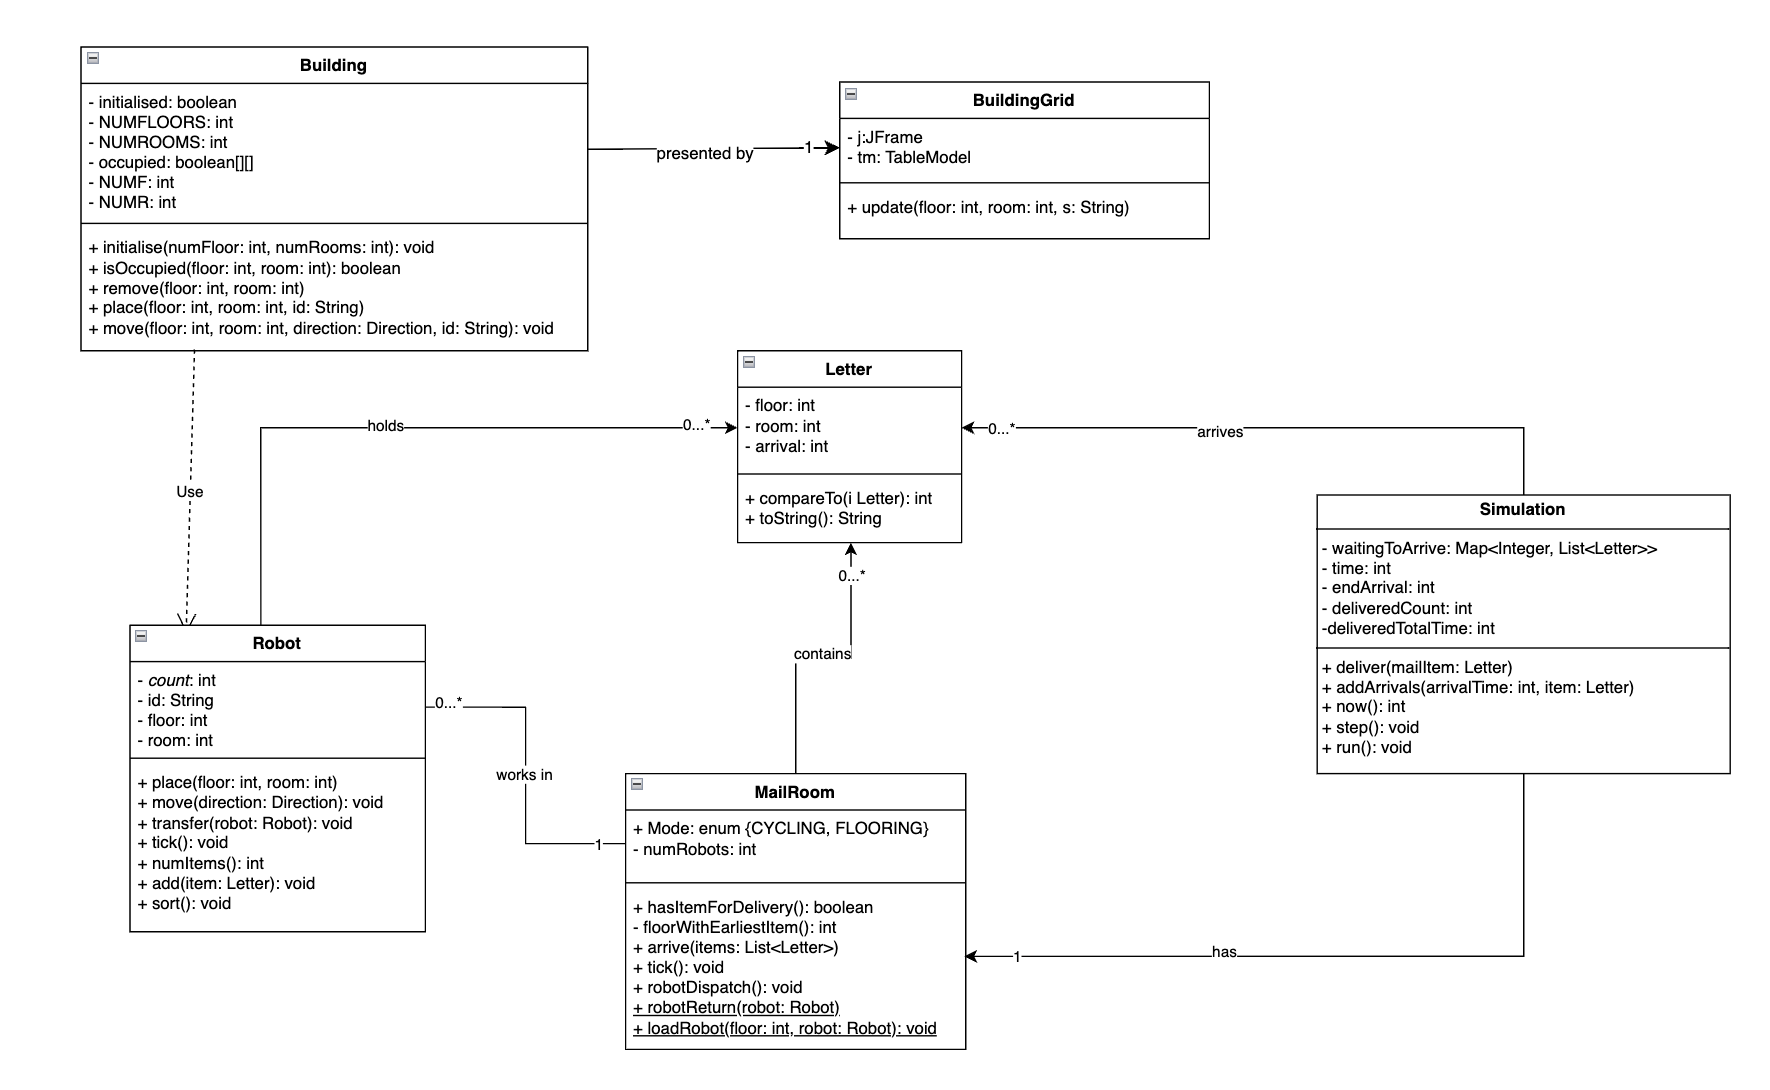
\includegraphics[width=1\linewidth]{Original Design.png}
    \caption{The original Design of AutoMail System}
    \label{fig:enter-label}
\end{figure}

\subsection{Advantages of Original Design}
\begin{enumerate}
    \item \textbf{Singleton Design} for the Building Class:
    \begin{enumerate}
        \item \textbf{Global Access Point}: The Singleton pattern provides a global access point to the Building instance. This makes it easier to manage and coordinate activities within the building.
        \item \textbf{Efficient Resource Use}: By ensuring only a single instance of the Building exists, the system avoids unnecessary duplication of resources, thereby saving memory and processing power that would otherwise be consumed by multiple instances.
        \item \textbf{System-Wide Consistency}: The Singleton pattern guarantees that all components of the system operate on the same Building instance, thereby preventing inconsistencies that could arise from having multiple instances (e.g., conflicting room assignments or occupancy data).
    \end{enumerate}
\end{enumerate}

\subsection{Disadvantages of Original Design}
\begin{enumerate}
    \item \textbf{High Coupling }Between Classes:
    \begin{enumerate}
        \item \textbf{Robot and Building}: The Robot class has a direct dependency on the Building class, leading to high coupling. This high coupling reduces the system's flexibility and maintainability. For instance, any modifications to the Building class may necessitate corresponding changes in the Robot class. Additionally, the Building class contains methods like \textit{move}, which may overlap with the responsibilities of the Robot class, potentially leading to redundant code and further complicating maintenance.
        \item \textbf{MailRoom and Simulation}: The MailRoom class is directly associated with both the Robot and Simulation classes. While some interaction is necessary, the direct and potentially complex relationships between these classes can make the system more difficult to understand, maintain, and extend.
    \end{enumerate}
    \item \textbf{Low Cohesion} Within Classes:
    \begin{enumerate}
        \item \textbf{Building} Class: The Building class is burdened with a wide range of responsibilities, including managing robot movements, which could be seen as unnecessary. This broad scope reduces cohesion, making the Building class harder to manage and more prone to errors.
        \item \textbf{MailRoom} Class: According to the system's specification, the MailRoom should primarily manage items. However, in the original design, the MailRoom class is also responsible for managing robots, which dilutes its cohesion and deviates from its intended role.
    \end{enumerate}
    \item \textbf{Scalability} Concerns:
    \begin{enumerate}
        \item \textbf{Handling New Modes} (e.g., FLOORING Mode): The original design does not easily accommodate the addition of new modes such as the FLOORING mode. For example, since the MailRoom class directly manages robot operations, introducing new behaviors or modes would likely require significant changes to the existing code, making the system less scalable.
    \end{enumerate}
    \item \textbf{Inheritance vs. Composition}:
    \begin{enumerate}
        \item \textbf{Robot and Item (Letter/Parcel)} Classes: The original design lack of the use of inheritance to manage different types of robots or items (e.g., Letter, Parcel), this leads to less flexible if there are more types of items or robots are introduced in.
    \end{enumerate}
\end{enumerate}

\newpage

\section{Refactoring, Improvements and Extension}
\setlength{\parindent}{2em} As shown in Figure 1, the original design has been significantly improved by applying GRASP (General Responsibility Assignment Software Patterns/Principles).
\begin{figure}[H]
    \centering
    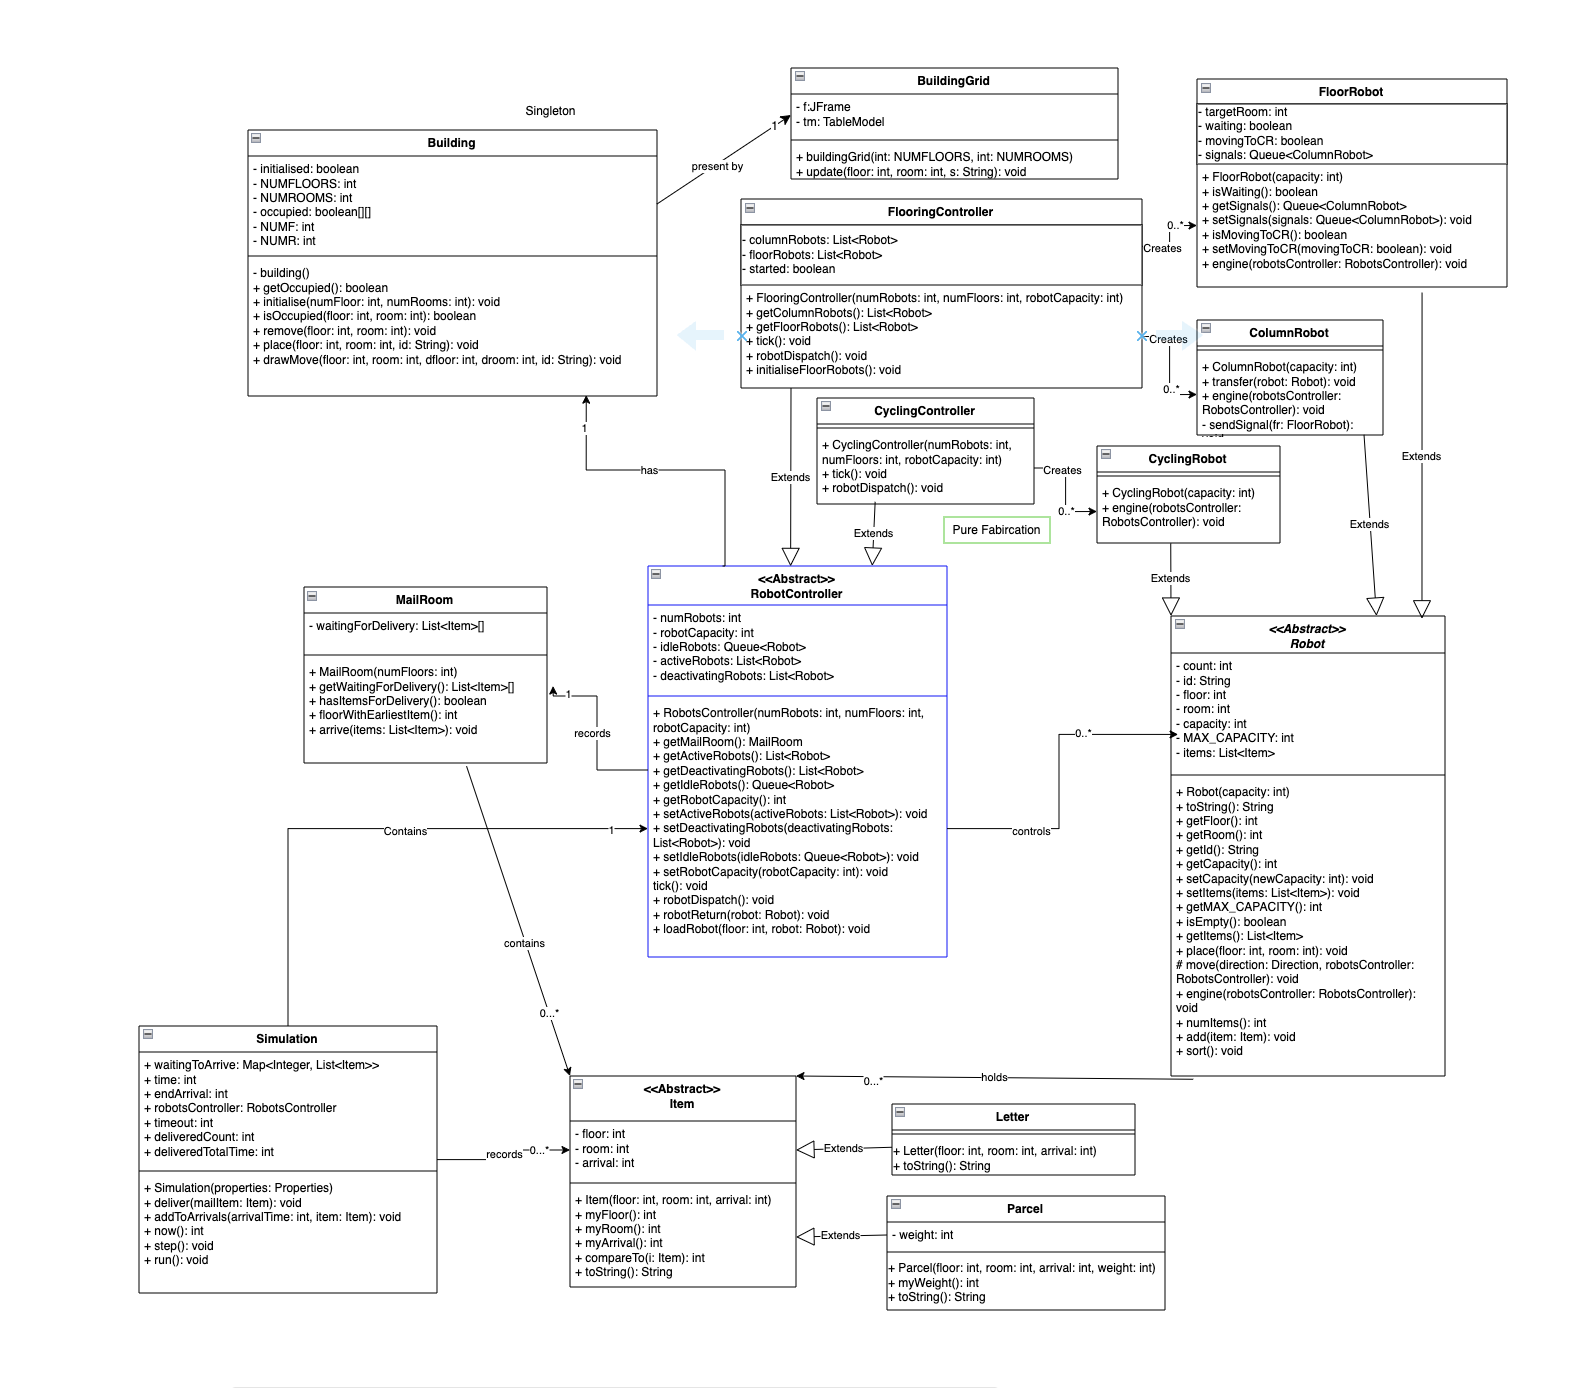
\includegraphics[width=1\linewidth]{Current Design.png}
    \caption{Design After Improvement}
    \label{fig:enter-label}
\end{figure}

\subsection{Use of Pure Fabrication and Indirection:}
\begin{enumerate}
    \item \textbf{RobotController Class}: To reduce direct coupling between key classes in the system, such as Robot and Building, and MailRoom and Simulation, we introduced the RobotController class. This class serves as an indirection layer and is a prime example of Pure Fabrication. The RobotController manages the responsibilities that were previously spread across the Building and MailRoom classes, leading to poor cohesion in those classes.
    \item \textbf{Improved Cohesion}: By transferring these responsibilities to RobotController, we improved the cohesion of both the Building and MailRoom classes. Now, each class has a clearer, more focused set of responsibilities, enhancing the system's maintainability and scalability.
\end{enumerate}

\subsection{Application of the Creator Principle:}
\begin{enumerate}
    \item \textbf{RobotController as the Creator}: In our redesigned system, the RobotController class is responsible for creating instances of Robot. This responsibility assignment aligns with the Creator principle and significantly increases the cohesion within the RobotController. By centralizing robot creation, RobotController can efficiently manage and coordinate robot behaviors without relying on external classes, thereby reducing coupling and enhancing the overall structure.
    \item \textbf{Simulation as the Creator of Items}: Similarly, the Simulation class is tasked with creating instances of Items, such as Letter and Parcel. This design choice ensures that the Simulation class maintains control over the lifecycle of items within the system, leading to higher cohesion within the Simulation class. By adhering to the Creator principle, the system becomes more modular and easier to extend, as each class has clear responsibilities for creating and managing specific entities.
\end{enumerate}

\subsection{Adherence to the Information Expert Principle:}
\begin{enumerate}
    \item \textbf{Encapsulation of Responsibilities}: By introducing the RobotController as an intermediary class, we ensured that each class in our redesigned system adheres to the Information Expert principle. For example, in our original design, the MailRoom class handled not only mail item management but also some aspects of robot coordination, which diluted its focus. By shifting robot-related responsibilities to the RobotController, the MailRoom class now exclusively manages mail item deliveries, ensuring it handles only the information it is directly responsible for. Similarly, the Building class no longer manages robot movements directly, which is now within the scope of the RobotController, further streamlining the responsibilities across the system.
    \item \textbf{Focused Responsibility}: In the redesigned system, the RobotController handles all robot-related operations, such as robot dispatch, return, and task assignment, which were previously scattered across different classes. This change enhances the cohesion of the RobotController by centralizing all robot-specific logic within one class. The Building, MailRoom, and Simulation classes now focus solely on their core responsibilities: Building manages structural aspects like floors and rooms, MailRoom oversees the queue and sorting of mail items, and Simulation manages the overall system flow and timing. This clear separation ensures that each class operates independently and efficiently, reducing the likelihood of cross-class dependencies and making the system more maintainable and extendable.
\end{enumerate}

\subsection{Application of Polymorphism}
\begin{enumerate}
    \item Polymorphism in \textbf{Item}, \textbf{Robot}, and \textbf{RobotController} Classes: To effectively manage the different cases and modes within the system, we employed polymorphism and inheritance across the Item, Robot, and RobotController classes. This design choice allows for a more flexible and extensible system, where behaviors can vary dynamically based on the specific subclass being used.
    \item \textbf{Item Class Hierarchy}: The Item class serves as an abstract base class for both Letter and Parcel. By utilizing inheritance, we can encapsulate shared attributes and methods within the Item class while allowing Letter and Parcel to extend and customize their behavior as needed. This approach reduces code duplication and promotes code reuse, ensuring that any changes to the common behavior are centralized in the Item class, making the system easier to maintain.
    \item \textbf{Robot Class Hierarchy}: Similarly, the Robot class is an abstract base class for various types of robots, such as CyclingRobot, FloorRobot, and ColumnRobot. Each robot subclass can implement specific behaviors and responsibilities, such as how they move or interact with items. Polymorphism allows the RobotController to interact with any type of robot without needing to know the specifics of each type, thus promoting flexibility and reducing the complexity of the RobotController class.
    \item \textbf{RobotController and its Subclasses}: The RobotController class itself is abstract, with specific controllers like CyclingController and FlooringController extending it. This design allows each controller to manage a specific mode or type of robot, encapsulating the logic required for that mode. This not only makes the code more modular but also simplifies the addition of new modes in the future, as new controllers can be created without modifying the existing ones.
\end{enumerate}

\subsection{Implementation of the Flooring Mode:}
\begin{enumerate}
    \item Using the design principles discussed above, we successfully implemented all the requirements for the Flooring mode. The following sequence diagram illustrates the process where a ColumnRobot loads items from the MailRoom, sends a signal to a FloorRobot, transfers the items to the FloorRobot, and finally, the FloorRobot delivers the items.
\end{enumerate}

% 这里加上一个Design sequence diagram的图片

\newpage

\section{Future Development Plan}
\setlength{\parindent}{2em} 
To ensure our design remains extendable and adaptable for future development, we have incorporated the following:

\subsection{Application of the Factory Pattern:}
Discuss how the system can be extended to support multiple machines of each type, along with any architectural changes required.
\begin{figure}[H]
    \centering
    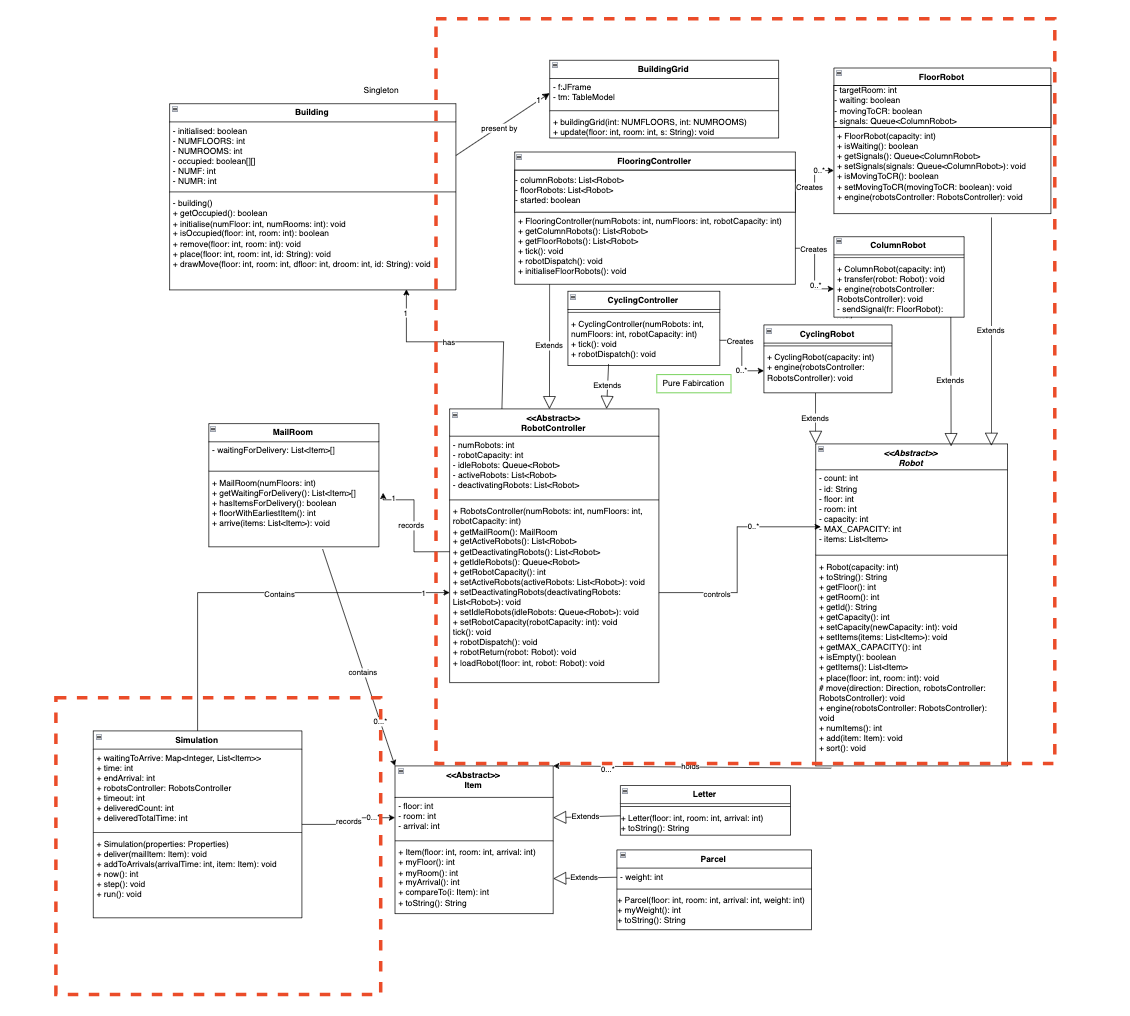
\includegraphics[width=1\linewidth]{Factory Pattern.png}
    \caption{Factory Pattern Applied in Our Design}
    \label{fig:enter-label}
\end{figure}
\begin{enumerate}
    \item \textbf{Encapsulating Object Creation}: The Factory Pattern is utilized to create objects—specifically, the RobotController and its associated Robot types—without specifying the exact class of object to be instantiated. This pattern allows us to encapsulate the object creation process, enabling the system to produce different types of objects based on the input criteria, such as the operational Mode.
    \item \textbf{Switch Statement in the Simulation Class}:
    \begin{enumerate}
        \item Within the Simulation class, a switch statement is employed to determine the operational Mode and instantiate the appropriate RobotController, either CyclingController or FlooringController.
        \item This aligns with the Factory Pattern as it abstracts the creation logic of the RobotController objects, making the Simulation class more modular and adaptable to future changes.
    \end{enumerate}
    \item \textbf{RobotController Creating Relevant Robots}:
    \begin{enumerate}
        \item Once the specific RobotController is instantiated, it is responsible for creating the relevant types of robots, such as CyclingRobot, FloorRobot, or ColumnRobot. This setup allows each RobotController to act as a factory, producing the necessary robot instances required for its respective mode.
        \item This design is a clear application of the Factory Pattern, where the factory (the RobotController) creates the objects (Robots) needed by the client (the Simulation class).
    \end{enumerate}
    \item \textbf{Benefits of this Design}:
    \begin{enumerate}
        \item With this implementation, the Simulation class functions as a client that leverages a factory (the switch block) to generate different types of RobotController. These controllers, in turn, create the specific Robot instances needed for the selected mode.
        \item This approach encapsulates the object creation process, providing the flexibility to add new modes or robot types in the future without requiring significant changes to the client code. This makes it a robust example of the Factory Pattern in action, contributing to the system's extendability and maintainability.
    \end{enumerate}
\end{enumerate}

\section{Conclusion}
In conclusion, the refactoring and extension of the Automail System have significantly improved its design, making it more cohesive, flexible, and ready for future enhancements. By implementing the FLOORING mode, we demonstrated how the system could be extended to accommodate more complex behaviors while maintaining maintainability and scalability. The application of design patterns like the Factory Pattern and GRASP principles has not only solved existing design issues but also laid a strong foundation for future development. Moving forward, the system is well-positioned to adapt to new requirements, such as the introduction of additional robot types or operational modes, with minimal impact on the existing codebase.

\end{document}
